\chapter{Testing della scheda}

Terminato l’assemblaggio, siamo passati alla fase di testing, in cui abbiamo verificato il funzionamento delle schede in tutti i loro aspetti.
Anzitutto abbiamo provato ad alimentarle via USB per verificare che la regolazione di tensione fosse funzionante. Abbiamo sfruttato il led sulla rail dei 3.3V come indicatore principale, poi abbiamo effettuato una misura più accurata tramite multimetro, appurando che il dimensionamento è stato fatto in modo corretto. Infatti sul testpoint della rail abbiamo misurato $3.3V \pm 0.05V$. \\
Dopo aver appurato che l’alimentazione fosse funzionante abbiamo flashato il microcontrollore con il codice che abbiamo sviluppato in parallelo su una \textit{dev-board Raspberry Pi Pico} ed abbiamo verificato il corretto assemblaggio dei componenti. \\
Con un programma di prova abbiamo poi applicato un segnale di controllo ai motori e, analizzando l’uscita dello stadio con l’oscilloscopio, ci siamo accorti che in uscita non si aveva il segnale desiderato. Perciò prima abbiamo testato il segnale \textit{PWM} generato dal microcontrollore, il quale è risultato corretto. Poi siamo passati al test sui \textit{mosfet} di pilotaggio. Qui ci siamo accorti che il segnale era sbagliato, quindi abbiamo intuito che il problema fossero i transistor. Il professore ci ha poi aiutati a capire nel dettaglio il problema misurando la tensione ai capi del diodo di protezione tra drain e source del \textit{mosfet}. Risultando un cortocircuito tra drain e source abbiamo capito che quelli non erano realmente il drain e il source del \textit{mosfet}x e ci siamo accorti che, in fase di progetto, ai transistor a canale N montati sulla scheda era stata assegnata la piedinatura scorretta. Effettuando la misurazione di tensione tra i vari pin del transistor abbiamo capito quale fosse il gate ed abbiamo provveduto a dissaldare e risaldare i transistor nella posizione corretta. Dopo questa correzione il sistema di pilotaggio degli stepper è risultato funzionante.
I restanti componenti sono stati testati con diverse iterazioni del \textit{firmware} e sono risultatI perfettamente funzionanti. \\
Per concludere abbiamo misurato il consumo del prototipo all’avviamento dei motori e in modalità idle,  ricavando le seguenti misure:

\begin{itemize}
    \item consumo a motori attuati: $<1.2 W$;
    \item consumo in idle: $<0.25 W$;
\end{itemize}
I consumi totali risultano complessivamente bassi poiché, data l'elevata coppia statica dei motori, non è necessario alimentarli per tenerli in posizione fissa.

\begin{center}
    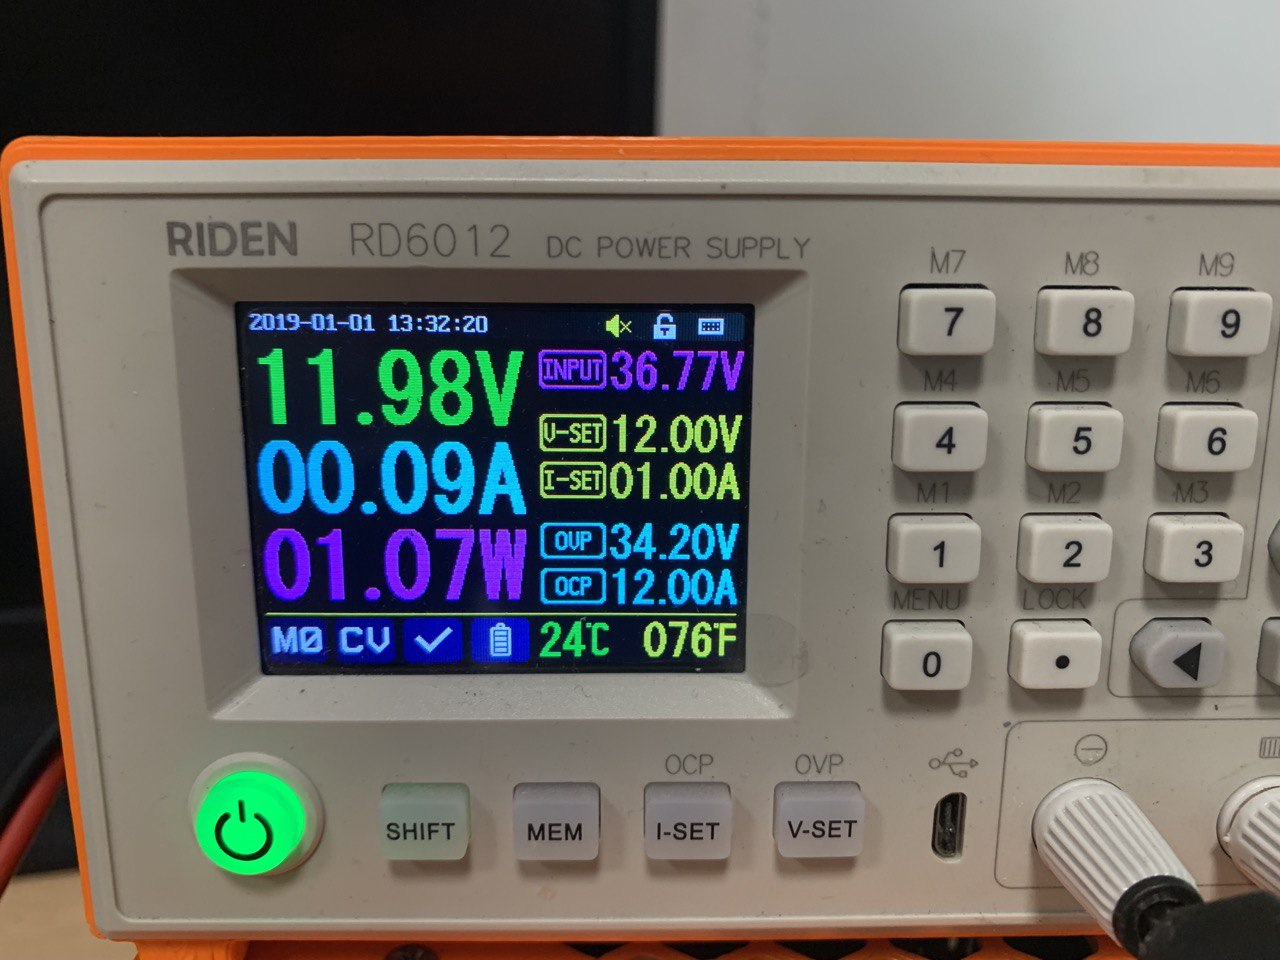
\includegraphics[width=10cm]{figures/image3.png}
    \captionsetup{type=figure}
    \captionof{figure}{Consumi durante il movimento dei motori}
\end{center}

\begin{center}
    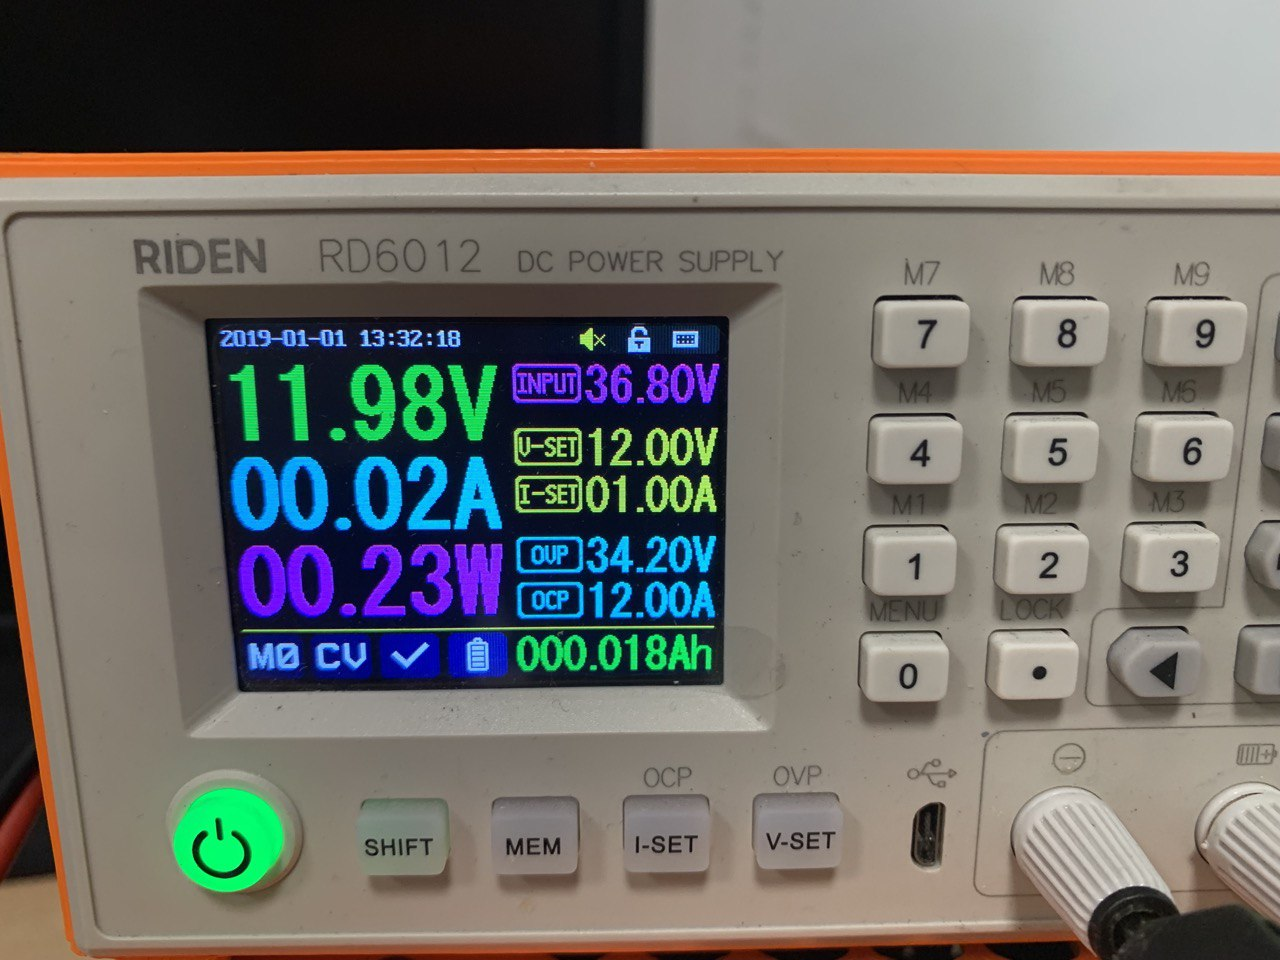
\includegraphics[width=10cm]{figures/image1.png}
    \captionsetup{type=figure}
    \captionof{figure}{Consumi durante lo stato di idle}
\end{center}

\begin{center}
    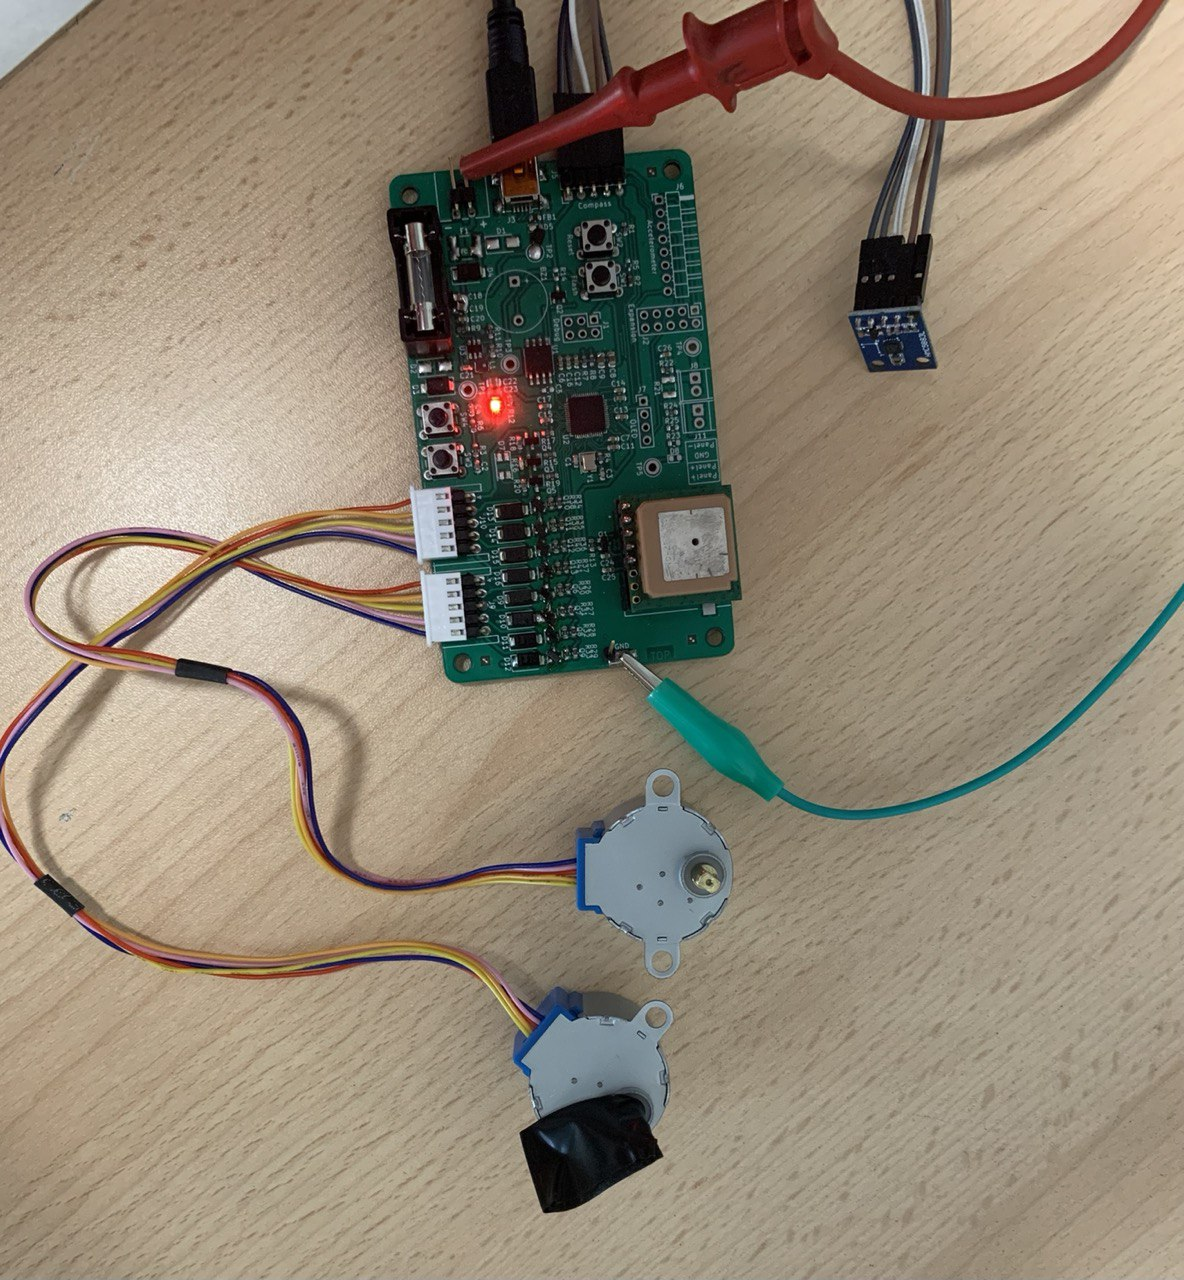
\includegraphics[width=15cm]{figures/image101.png}
    \captionsetup{type=figure}
    \captionof{figure}{La scheda in fase di testing}
\end{center}
